\chapter{Sci-Genie Core}
\label{sci-genie-core}
\begin{figure}[p]
    \centering
    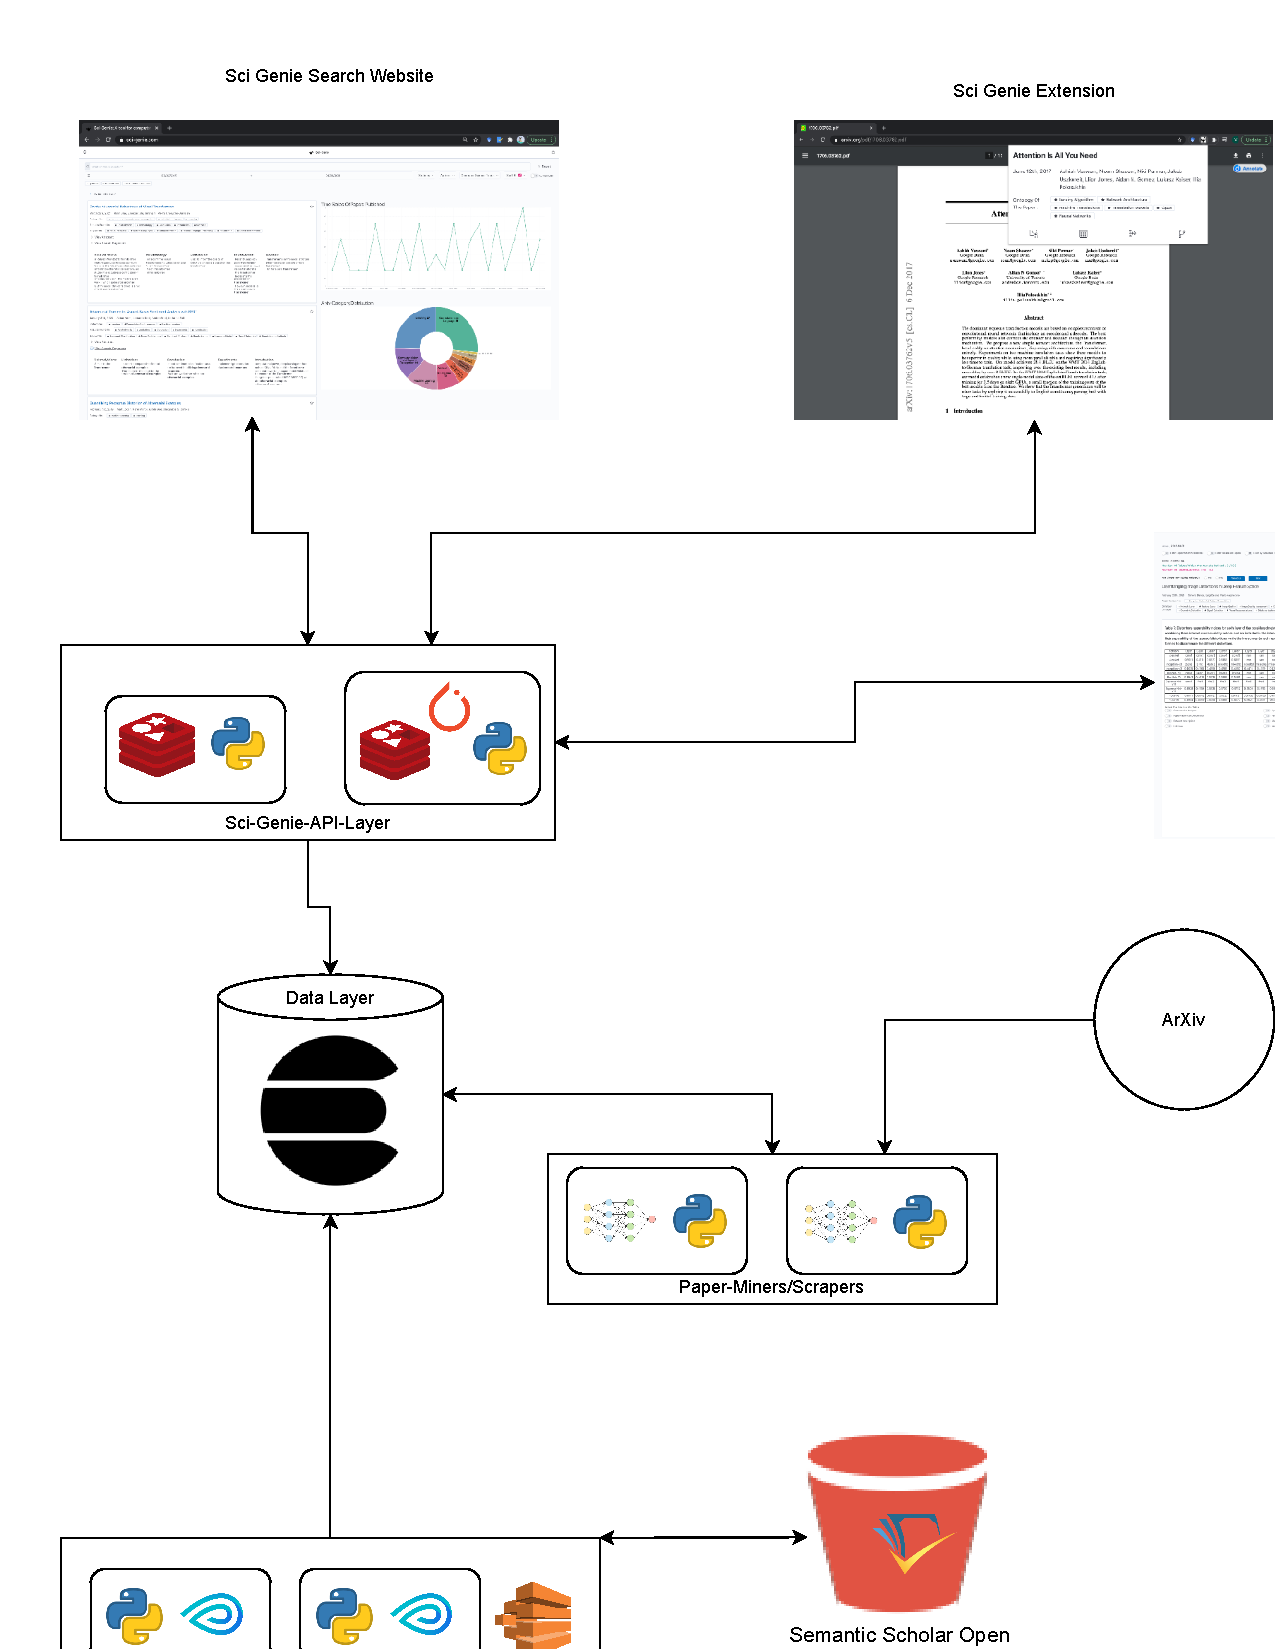
\includegraphics[width=\maxwidth{\textwidth}]{src/images/Sci-Genie-Arch.pdf}
    \caption{Sci-Genie System Architecture}
    \label{figure\arabic{figurecounter}}
\end{figure}
\refstepcounter{figurecounter}
% \pagebreak

\section{System Architecture}

Sci-Genie Core comprises four key architectural components which help power information for multiple different apps like the browser-extension, the website and the labeling interfaces for machine learning. 
\begin{itemize}
    \item \textbf{Data Layer}
    \item \textbf{API Layer}
    \item \textbf{Paper Scraping And Mining Engine}
    \item \textbf{Semantic Scholar Citation Graph Mining Engine}
\end{itemize}

Paper Scraping And Mining Engine help extract papers From ArXiv in LaTeX format and then parses the structure, mines the ontology, and extracts the tables. The processed information gets stored in the Data Layer. 

The Data Layer hosts the information used by the website or the browser extension. 

The Semantic Scholar Citation Graph Mining Engine leverages a data processing pipeline to filter CS research and create an index in the Data Layer, containing information corresponding to citations of papers from ArXiv. 

The API Layer leverage the general-purpose abstractions built around the Data Layer to access and further intelligently process information at search time. The API Layer connects the Data Layer with various applications like The Sci-Genie Website, The Sci-Genie extension and other apps such as the Table Labeling tool. 

\section{Sci-Genie Data Layer}
\label{sci-genie-core:data-layer}
The Data Layer comprises the open-source search engine named Elasticsearch\parencite{gormley2015elasticsearch} which is built on top of Lucene. 
The data layer aims to host processed information after scraping, mining, and parsing research documents and tables. 
Elasticsearch hosts the following indexes\footnote{Index is similar to Database in the language of RDBMS}\footnote{https://www.elastic.co/guide/en/elasticsearch/reference/current/documents-indices.html} to filter access of content:
\begin{itemize}
    \item \textbf{Arxiv Parsed Research Index}:\textit{Contains research documents whose structure is explicitly parsed and stored}
    \item \textbf{Semantic Scholar Index}:\textit{Contains documents from the CS Domains mined and filtered from semantic scholar open research corpus}
    \item \textbf{Arxiv Table Index}:\textit{Stored the tables from research papers which can be later used for information augmentation.}
    \item \textbf{Arxiv Semantic Scholar Join Index}:\textit{Stores the citation information filtered from semantic scholar index to map papers in ArXiv} 
\end{itemize} 

\subsection{Arxiv Parsed Research Index}

Documents in the Arxiv Parsed Research Index helps power the search for the Sci-Genie search website. All documents belong to Computer Science ArXiv and 
the construction of these documents is discussed in Section \ref{sci-genie-core:scraping}. Each document consists of three 
key pieces of information:
\begin{itemize}
    \item \textbf{ArxivIdentity} \textit{ArXiv associated meta-data information}
    \item \textbf{ResearchObject} \textit{Parsed Research structure}
    \item \textbf{Ontology} \textit{Ontology belonging to the article.}
\end{itemize}

\subsubsection{ArxivIdentity}
ArXiv associated meta-data information holds information regarding the abstract, title, authors, categories of the paper etc. 
The information stored in this object helps provide search stratagems to the Sci-Genie search website. 

\subsubsection{ResearchObject}
\label{sci-genie-core:data-layer:researchobj}
The ResearchObject is the data structure that holds the parsed text from the research document. 
The purpose of this object is to fit the research document and its hierarchy into predefined sections
which are commonly occurring in research documents. The general pre-identified sections are given below:
\begin{itemize}
    \item Introduction
    \item Related Works
    \item Methodology
    \item Experiments
    \item Results
    \item Dataset
    \item Conclusion
    \item Limitations
\end{itemize} 
Any section that doesn't fit the predefined sections will be categorized as \textit{Unknown}. 

The ResearchObject consists of key value pairs which relate to the given predefined sections. The key is the name of the section eg. Introduction, Related Works etc. and the value is a \textit{Fragment}. 
Fragment is a tree-like data structure that holds hierarchical information. Fragment is given by:
\begin{verbatim}
    class Fragment:
        title:str = "Introduction"
        text:str = "Text relating to the introduction of a paper"
        children:List[Fragment] 
\end{verbatim}    

The \textit{children} in the Fragment hold the information about the child notes of that Fragment. The Fragment object helps capture a research paper’s hierarchy before it gets parsed into a key-value-based ResearchObject. The Fragment object can also be serialized to JSON making it indexable in the Lucene search index.  

Due to the search engine’s scope being limited to CS research on ArXiv, the predefined sections are created based on a statistical analysis of the content after scraping. Section \ref{sci-genie-core:scraping} provides more details on the creation of the Fragment and ResearchObject. 

\paragraph{Advantages Of Indexing ResearchObject}
The ResearchObject is a key value-based object, and each key allows indexing the text according to its corresponding section. This object schema helps provide more context about the search match within each section, as seen from Figure \ref{figure7}. 

\subsubsection{Ontology}
\begin{figure}[h]
    \centering
    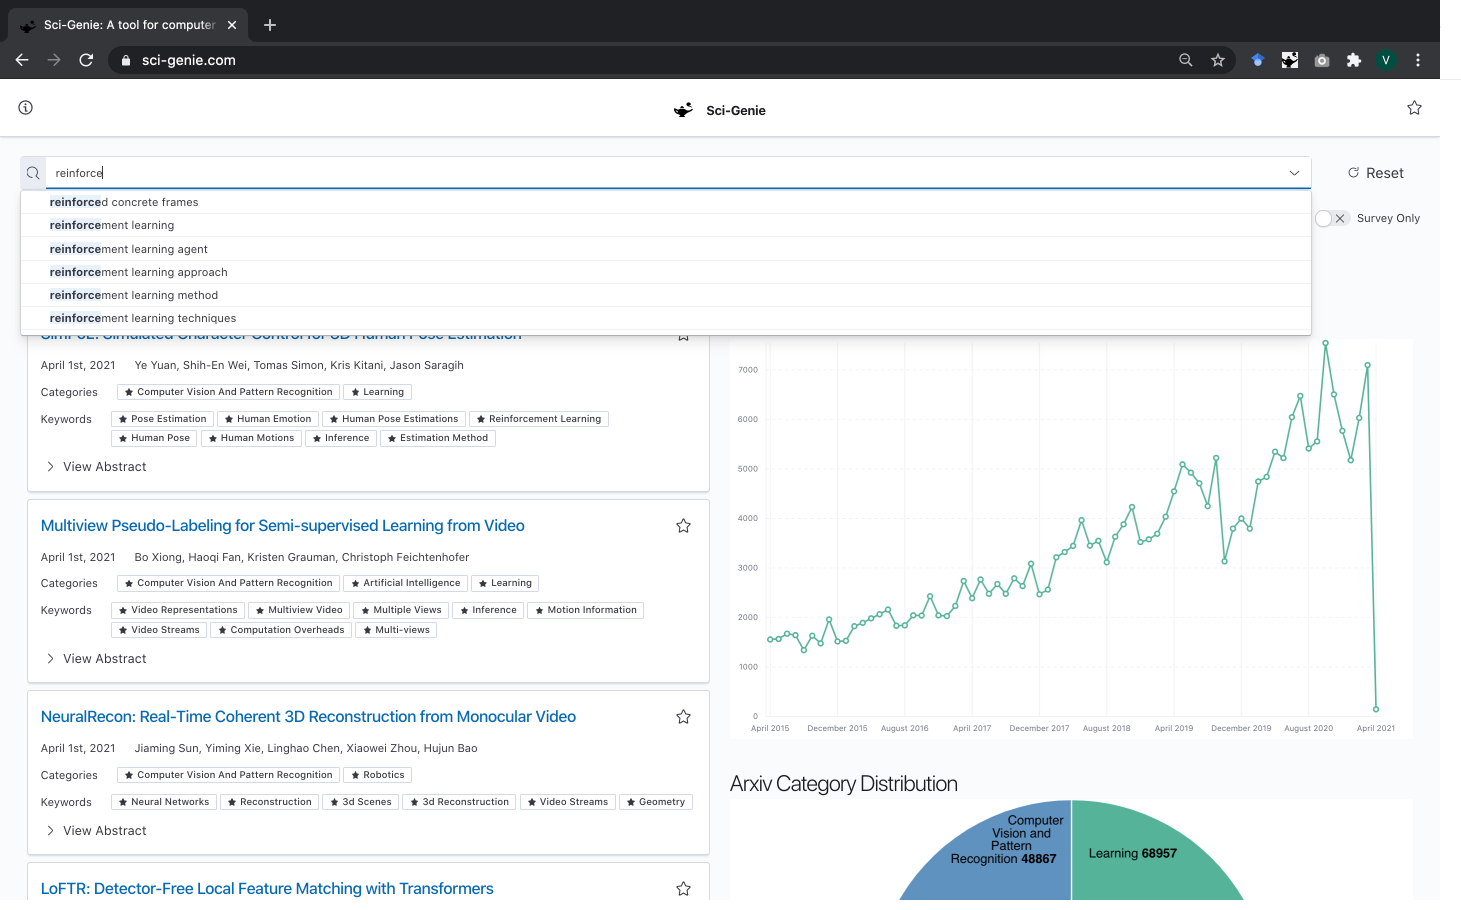
\includegraphics[width=\maxwidth{\textwidth}]{src/images/sci-genie-autocomp-example.png}
    \caption{Sci-Genie auto-completing the search terms using the ontology}
    \label{figure\arabic{figurecounter}}
\end{figure}
\refstepcounter{figurecounter}

The study conducted by \cite{li2017investigating} gave a great indicator regarding the need for entity based queries in academic research search engines to improve precision. As Sci-Genie only operates over computer science research, the research papers’ ontology helps power the autocomplete panel in the search bar from Figure \ref{figure13}. Each paper consists of an ontology which is classified via CS specific ontology classifier.\footnote{https://github.com/angelosalatino/cso-classifier\#sample-output-sp}. Sci-Genie indexes the entire ontology given by \cite{salatino2020ontology}. 

\subsection{Semantic Scholar Index}
\label{sci-genie-core:data-layer:ss-index}
This index hosts information filtered from the Semantic Scholar Open Research Corpus\parencite{ammar-etal-2018-construction} post Citation Graph Mining. More details on how it is filtered is described in Section \ref{sci-genie-core:citation-mining}. This index’s core purpose is to help correlate citation to and from papers on ArXiv. The Sci-Genie extension further uses this citation information for finding tables from the neighborhood of papers as seen in Figure \ref{figure9}. 


\subsection{Arxiv Table Index}
\label{sci-genie-core:data-layer:table-index}
This index holds information regarding the tables from a research paper. The core methodology which is used to extract and serialize/deserialize tables from LateX is based the methodology developed by \cite{kardas2020axcell}. The method created by  \cite{kardas2020axcell} helps convert tables in pandas\footnote{https://pandas.pydata.org/} serializable DataFrames. These DataFrames can be serialized to json for storage in Elasticsearch. The schema for the object can seen below : 
\begin{verbatim}
    class ArxivTable:
        semantic_scholar_id:str = ""
        arxiv_id:str=""
        identity:str = ""
        figure_id:str=""
        caption:str=""
        name:str=""
        layout:str=""
        table:str=""
\end{verbatim}

The \textit{identity} is the unique identifier for a table. Each record also holds loose relations to the Arxiv Parsed Research Index and the Semantic Scholar Index via respective ids. 

\subsection{Arxiv Semantic Scholar Join Index}
\label{sci-genie-core:data-layer:ss-join-index}
This index holds references of in and out citations for each ArXiv article present in the Arxiv Parsed Research Index. Although the Semantic Scholar Index contains citation data, none of it is correlated with ArXiv articles and hence this index is created to help correlate information at search time. Below is the schema for the documents in the index: 
\begin{verbatim}
    {
        "in_citn_arxiv": [],
        "out_citn_arxiv": [],
        "semantic_scholar_id": "",
        "arxiv_id": "",
}
\end{verbatim}
The \textit{arxiv\_id} is the unique ArXiv identifier, The \textit{in\_citn\_arxiv} correspond to the unique ArXiv ids of papers that cited a paper. The \textit{out\_citn\_arxiv} correspond to the unique ArXiv ids of papers cited by a paper. This information comes of great use when filtering out tables as seen in Figure \ref{figure9}. The construction of this index is discussed in Section \ref{sci-genie-core:citation-mining}
% The ontology of research papers is stored in the same form as provided by the 
\section{Paper Scraping And Mining Engine}
\label{sci-genie-core:scraping}
The Paper Scraping And Mining Engine connects with ArXiv to extract LaTeX source data. The LaTeX source data undergoes three parallel processing steps:
\begin{itemize}
    \item Content Hierarchy Parsing : The extraction of content based on document structure for storage
    \item Ontology Mining : Correlating the ontology of the paper from ArXiv
    \item Table Extraction : Leveraging tools to extract tables from the ArXiv document's LaTeX source.
\end{itemize}

\subsection{Content Hierarchy Parsing}
A structured \nameref{sci-genie-core:data-layer:researchobj} is parsed from raw LateX content in two steps:
\begin{itemize}
    \item Step 1 : Extract the structure of the research document and create a Fragment object
    \item Step 2 : Correlate the children in the Fragment Object with predefined sections to create the \nameref{sci-genie-core:data-layer:researchobj} 
\end{itemize} 
\subsubsection{Fragment Creation}
\label{sci-genie-core:scraping:source-frag}
Each LaTeX source repository is parsed to create a "Structure Tree" of the research document. The Structure tree\footnote{https://github.com/alvinwan/tex2py} helps correlate the structure of latex document. The structure tree is then used to create Fragment objects described in Section \ref{sci-genie-core:data-layer:researchobj}. The text within each Fragment is populated by using the opendetex library\footnote{https://github.com/pkubowicz/opendetex}. The opendex library helps filter text information from individual tex files. The code to match the structure tree is provided in the Appendix. 

\subsubsection{ResearchObject Creation From Fragment}
\label{sci-genie-core:scraping:frag-to-rs}
The initial Fragment object created via the parsing described earlier will contain the entire research document stored in a single Fragment. This Fragment then undergoes a "heuristic" serialization to the ResearchObject. Meaning the title of the children within the Fragment is matched to predefined sections/classes given in Section \ref{sci-genie-core:data-layer:researchobj}. The matching process uses heuristics to match the content. More details on the section name matching strings and algorithm are given in the Appendix \ref{appendix:content-parsing-code} and \ref{appendix:mapping-heuristic} respectively. 

\subsection{Ontology Mining}
Sci-Genie leverages the ontology mining method described by the \cite{salatino2020ontology}. The research document's abstract and title are only needed for ontology mining. 

\subsection{Table Extraction and Storage}
To extract tables from papers on ArXiv, Sci-Genie uses arxiv-vanity/engrafo\footnote{https://github.com/arxiv-vanity/engrafo} to convert LaTeX to HTML and then employ table serialization methods created by \cite{kardas2020axcell}. The parsed tables are stored in the \nameref{sci-genie-core:data-layer:table-index}. 


\section{Semantic Scholar Citation Graph Mining.}
\label{sci-genie-core:citation-mining}
A rich source of context and metadata about the tables cited by a paper comes via the access to citations in a paper and leveraging the citation graph. The Semantic Scholar\footnote{http://s2-public-api-prod.us-west-2.elasticbeanstalk.com/corpus/} corpus consists of 136M research papers from various domains with their citations. This corpus event consists of all urls to a research paper, including the ones on ArXiv.  

Metaflow\footnote{https://metaflow.org/} is used to create a data processing pipeline\footnote{https://github.com/valayDave/semantic-scholar-data-pipeline} for filtering the subset of CS papers from the Semantic Scholar corpus. The filtered CS papers are stored in the \nameref{sci-genie-core:data-layer:ss-index}. 

The pipeline further correlates the citations of papers which are present on ArXiv and stores them in the \nameref{sci-genie-core:data-layer:ss-join-index}. 
% The Semani .

\section{API Layer}
The API layer is Sci-Genie, which leverages the general-purpose abstractions built over the DataLayer to access and process information for various apps such as the search engine website, the chrome plugin and the table labeling interface. 

\subsection{Scientific Table Correlation Via Citation Graphs}
With the access to distinctly processed and correlated information about research papers on ArXiv and their associated tables, the API Layer leverages these traits to filter tables from papers that cited the paper the user is reading (as seen in Figure \ref{figure14} and \ref{figure9}). 


\subsection{Table Of Comparison Classification}
\begin{figure}[h]
    \centering
    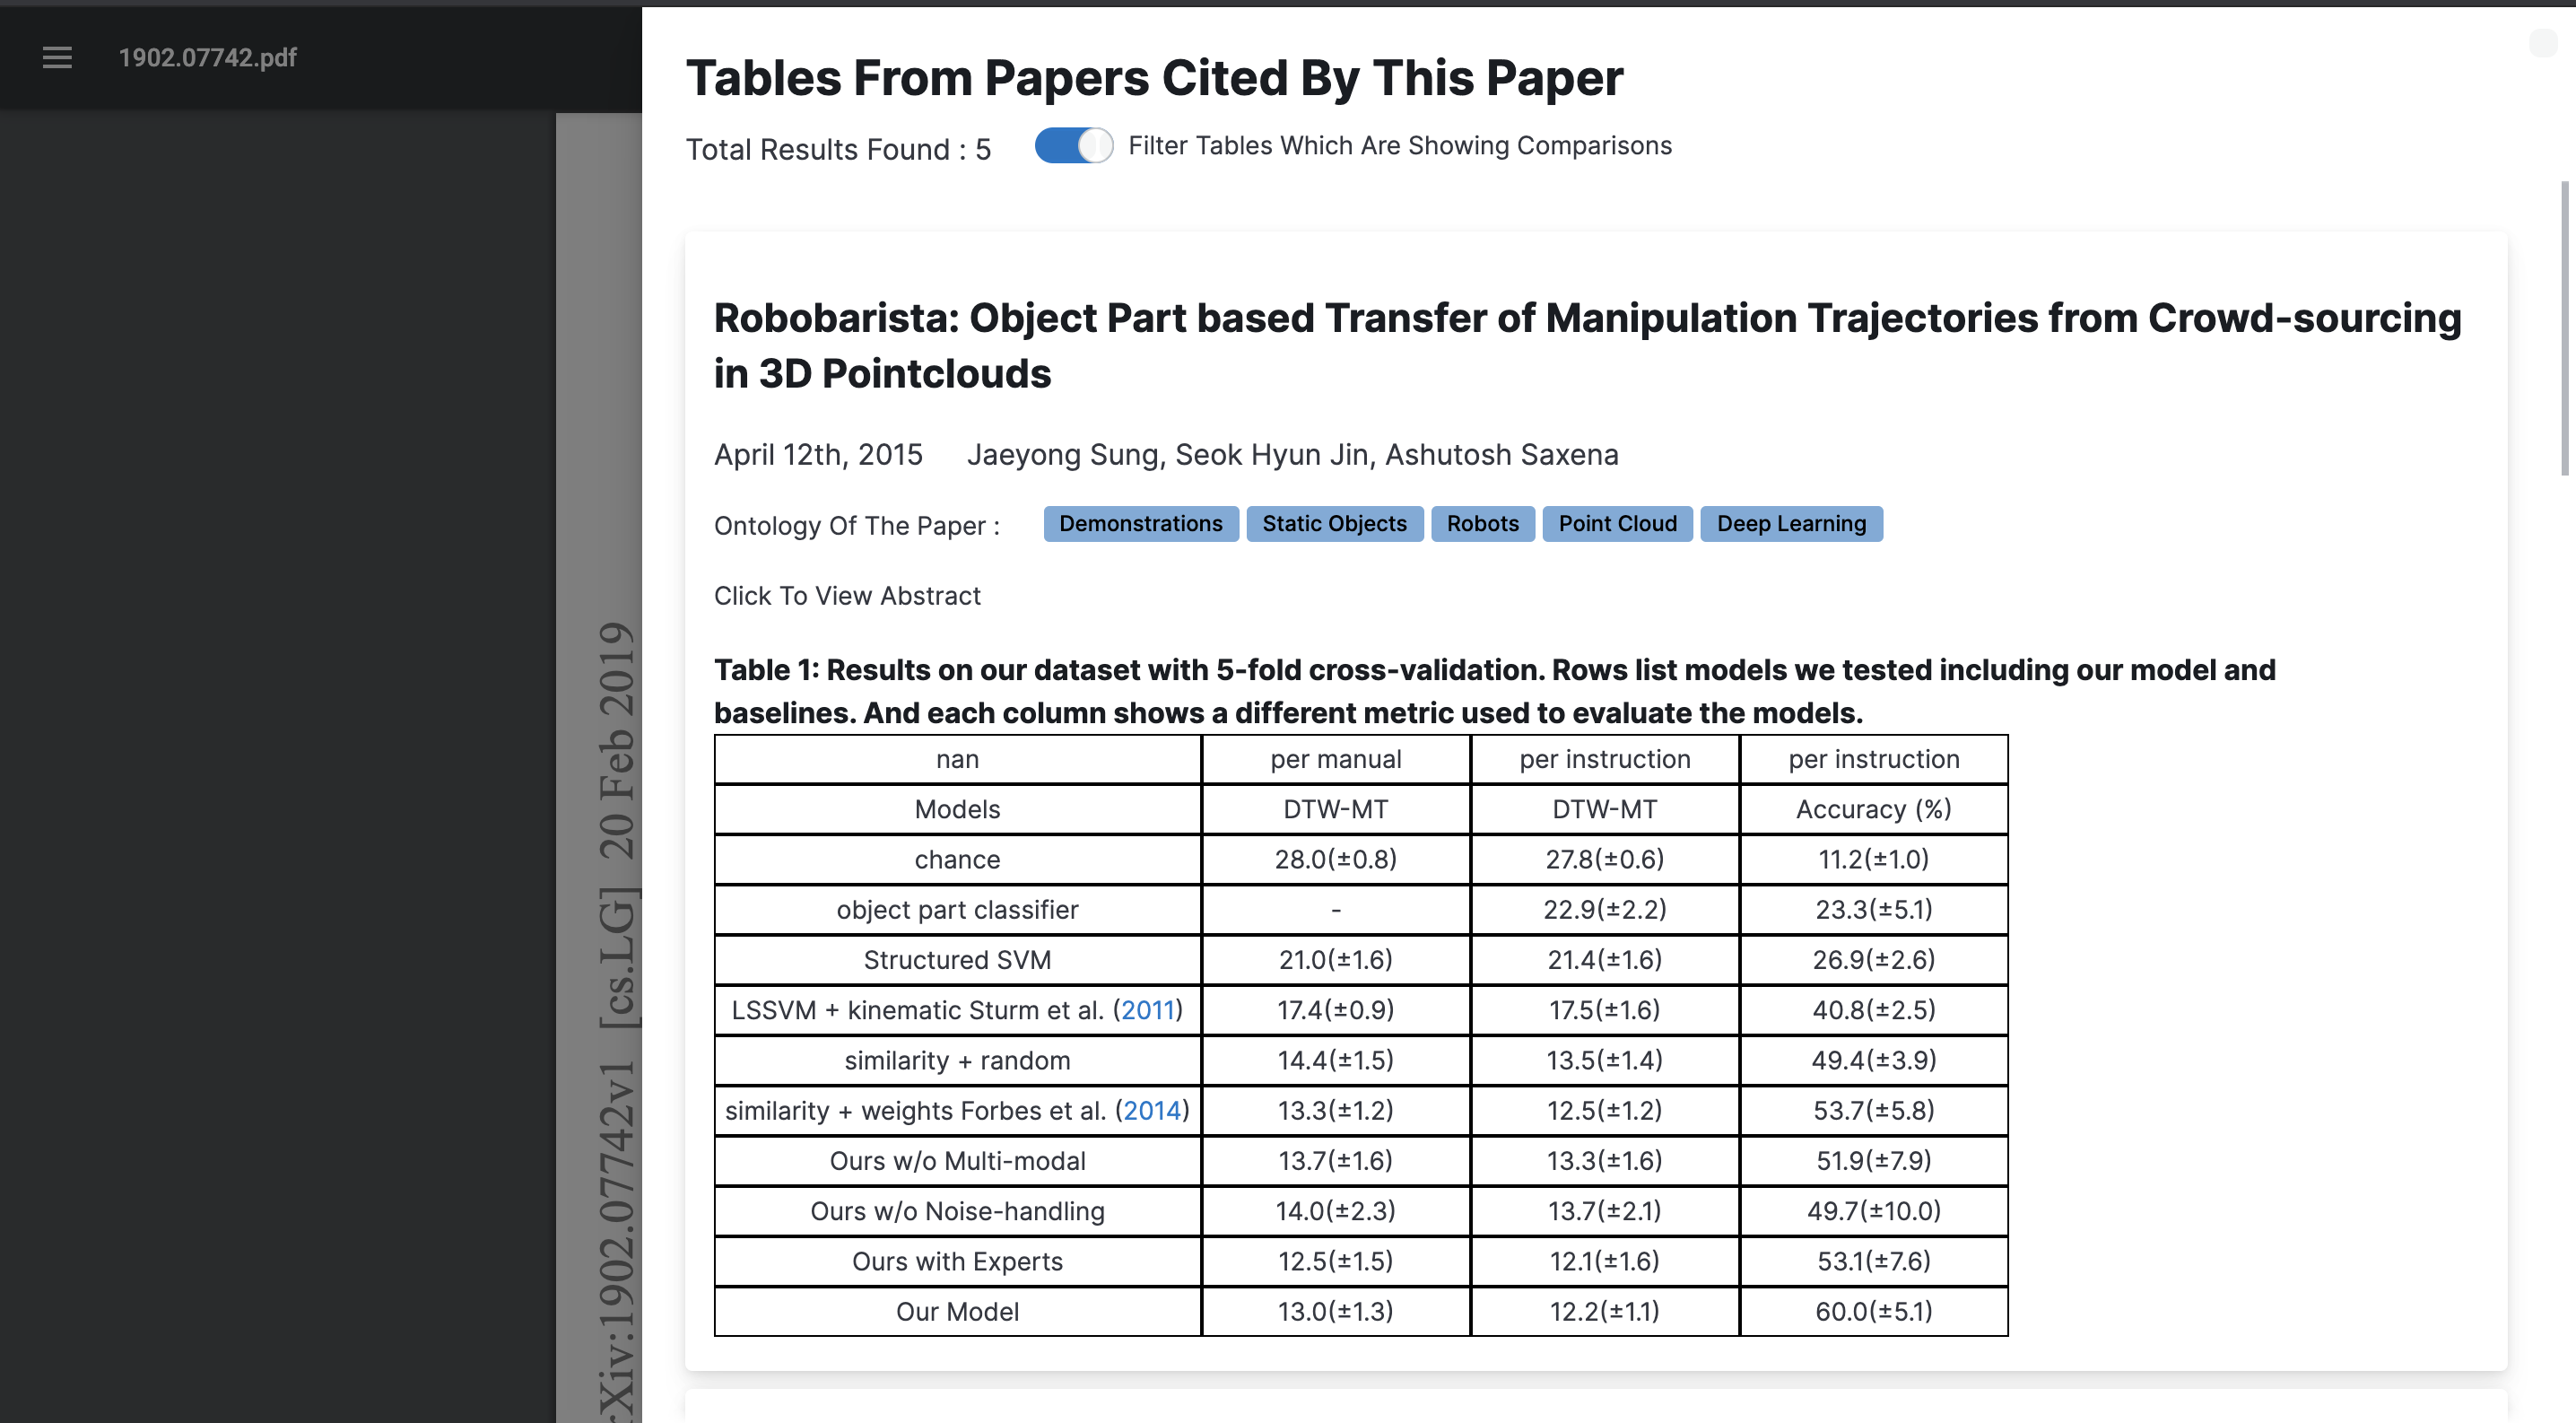
\includegraphics[width=\maxwidth{\textwidth}]{src/images/classification_exp.png}
    \caption{Tables describing comparisons filtered via API-Layer}
    \label{figure\arabic{figurecounter}}
\end{figure}
\refstepcounter{figurecounter}

The tables extracted from the papers that were cited also undergo a binary classification via a machine learning model to label the tables describing a comparison. This information is useful to provide context based filters at the time of reading, as seen Figure \ref{figure14}. Chapter \ref{table_classification} provides more details on the table of comparison classification and the choice of model for the API-Layer.
 
\subsection{Table Intent Labeling API}
The API Layer also provides API's for table annotation and labeling as seen in Figure \ref{figure15}. These annotations and labels help provide labeled data for the machine learning task which is discussed in Chapter \ref{table_classification}.

